
%=======================================================
\section{Use Case Analysis}
%=======================================================

%% come fanno ora la programmazione?
%% NG: oggi la programmazione viene portata avanti, nei singoli ospedali, in maniera autonoma e indipendente. In ogni presidio si riunisce un board chirurgico, più o meno settimanalmente. Durante questo incontro, oltre a linee di indirizzo, si conferma la distribuzione degli slot di sala (purtroppo questo rimane tracciato solo all'interno di file excel). Negli ultimi anni, se si vuole citare, abbiamo implementato un progetto di riorganizzazione (denominato HPR chirurgie 2.0) che era volto a studiare i percorsi nei singoli ambiti territoriali e riportare a tutta l'Azienda elementi di omogeneità, a riorganizzare la configurazione dell'offerta nei singoli ospedali e ad abilitare la lettura delle informazioni. Dopo circa un anno di lavoro si è distribuita una reportistica che - per la prima volta in AUSL Romagna - presenta la situazione quanto più reale possibile della lista di attesa chirurgica (circa 20.000 casi in attesa di chirurgia). Qui, se servono alcuni numeri, posso inserire: consistenza attuale (o media) della lista, numero di sale operatorie e numero di ospedali, produttività media, domanda media. Si potrebbe accennare al fatto che AUSL Romagna assiste un territorio che conta 1,125,0000 assistiti e la complessità deriva anche dalla disponibilità di 90 sale operatorie distribuite in 10 presidi molto differenti distribuiti nel territorio. Infine, per quanto riguarda il monitoraggio dell'efficienza delle sale operatorie in letteratura sono definiti indicatori specifici (utilizzo grezzo, utilizzo a valore, ritardi, anticipi, ...). Dalle cose che ho scritto qui, se ritenete utile alcuni elementi in particolare e mi dite quali, posso cercare dati e fonti (per questo o per l'estensione).

In collaboration with the Local Health Authority of Romagna, Italy (AUSL Romagna) we collected information about the current management of ORs across multiple hospitals and the needs expressed by both the on-site medical staff and the general administration in order to achieve better overall control without adding too much of a burden on the daily processes of all involved parties.

\subsection{Current Situation}
%due righe che incapsulano meglio il commento di Nicola qua sopra?

The current situation is not completely automated and relies on a QR code scanning system, a printed schedule of the planned surgeries for the day and a paper form for each surgery that is filled by hand by the medical staff.

The QR scanning system is designed to allow keeping track of the most relevant phases of a surgical procedure. These steps are the following:
\begin{enumerate}
    \item Patient exits the hospital ward
    \item Patient enters the operating suite
    \item Patient enters the OR\footnote{From now on if, for any unexpected reason, the surgical procedure is interrupted step 8 is the next one}  %% questo credo possa avvenire prima di Anesthesia performed, in generale. Esistono casi per i quali l'anestesia inizia fuori dalla sala operatoria, ma dipende dalla disponibilità o meno, nel blocco, di aree dedicate
    \item Anesthesia is performed\footnote{In some cases this step can happen before step 3 if there are dedicated facilities to support it}
    \item Anesthesia is effective
    \item Surgery is started
    \item Surgery is completed
    \item Patient is moved outside of the OR
    \item Patient leaves the operating suite
    \item Patient enters a hospital ward (which can be different from the one which he came from)
\end{enumerate}
%
After a surgical procedure, OR is cleaned and prepared for the next one. 

Timing of each step execution is also annotated on the paper form, steps that happen between since one of the main current issues is the discrepancy between the time the QR codes are scanned and the time steps are actually performed. This is due to the fact that the medical staff is usually very busy and focused on the patient and can forget to scan at the appropriate time. The paper form allows them to correct the timings annotating afterwards an estimated real-time based on what they remember doing as well as other relevant information about the surgery, which they may find useful to keep track of.

Another critical issue with the current state of the system is that data registered by the QR scanning system is stored in a database that is local to each hospital. This, of course, implies that the coordinators that need to manage the network of ORs are not able to automatically retrieve information about the current state of the ongoing surgical procedures, leading to less efficient management.

The main pain points that emerged in the conversation with the medical staff are here summarised:
\begin{itemize}
    \item Low readability of manually annotated data
    \item Limited space on the paper form to annotate surgery's steps
    \item Discrepancy between the scanned times and the real times
    \item Deletion or delay of planned surgery is currently not tracked since the schedule is printed
    \item Accountability for issues regarding data collection is impossible to define
    \item Sub-optimal management of OR due to the fact that the availability of a facility is not known in real-time
\end{itemize}

\subsection{Requirements}
From the analysis of the current situation and the staff needs the following functional requirements for a new management system are defined:
\begin{itemize}
    \item Real-time monitoring of the availability of ORs: whether they are busy at the moment and what the planned surgeries for each one are
    \item Time monitoring of surgical procedures and individual procedures' steps to understand the overall efficiency
    \item Automatic generation of warnings when there is inconsistency in the transmitted data (e.g. two patients in the same room at the same time, a step that is taking an unexpected amount of time)
    \item Storage of detected warnings for historical data analysis
    \item Easy data access through a dashboard to visualise the current state, review warnings, and annotate steps. The dashboard should also be accessed through an account to solve the problem of accountability.
\end{itemize}

From a more technical point of view, the new system was also required to be integrated with the existing solution, and to support interoperability with other future possible systems that may require access to data.

Note that the objective of this case study was not to completely revolutionise the current approach for OR management, but to improve it by adopting a DT based solution that opened the possibility of future expansion.

%=======================================================
\section{\acl{DTE} Proposal}
%=======================================================



The idea of applying the DT approach in the context of ORM that we put forth in this paper is based on the premises of Section~\ref{sec:background}: the need for efficient tools, possibly based on the most recent technologies, is clear and the DTs seems to provide all the required functionalities for effective scheduling of surgeries, as well as their management and supervision.  
%
They enable the acquisition of diverse data on the real system, the storing of all the historical information describing the evolution of its state, the encapsulation of a model for performing simulation and \textit{what-if} analysis, and finally, the inclusion of AI algorithms for reasoning on knowledge and data acquired, are all ingredients that can make the difference in this context.

In this section, we provide a description of an ecosystem of DTs devised for the operating suite and the surgical procedures performed.
%
Assuming to adopt DTs as a pervasive approach, we can envision having an ecosystem of connected DTs that can map real-world facilities.
%
Each hospital can have its own DT, connected to DTs of each OR which could be even connected to those of the medical equipment available in each room.
%
Similarly, we can mirror people, namely patients and the medical staff, into human DTs that are strongly interlinked with those of the facilities exploited.

The resulting network of DTs could represent the state of the healthcare system at any given time. For example, looking at the DT of a room and analysing the relationships with other DTs one could discover its planned and real-time availability, its equipment, the historical information about its management and so on.

In Fig.~\ref{fig:dt ecosystem} we show an example of how this ecosystem looks like. On top of that, a DT of each perioperative care path can be dynamically added and linked to other DTs in different phases of its lifecycle. 

When a doctor and a patient meet for an appointment and the need for a surgical procedure is identified \emph{(1)} a new \textit{Surgery DT} is created \emph{(2)} and linked to the DT of the patient \emph{(3)}. 
%
Then, whenever the surgery is scheduled in a specific room \emph{(4)} a relationship with the DT of that room is added to keep track of the planned surgeries per each room \emph{(5)}.

The patient is then usually hospitalised and transferred to the OR \emph{(6)}. When the patient actually enters the room the \textit{Surgery DT} creates a new relationship with the OR\footnote{for any reason it could also be a different room from the planned one} DT \emph{(7)} which will report that the room is actually busy.

Finally, when the patient leaves the room \emph{(8)}, the end time is registered -- e.g. by scanning a barcode like in our case study -- \emph{(9)} and the OR can now be set back to an available state after the necessary cleaning operations.

\begin{figure}
    \centering
    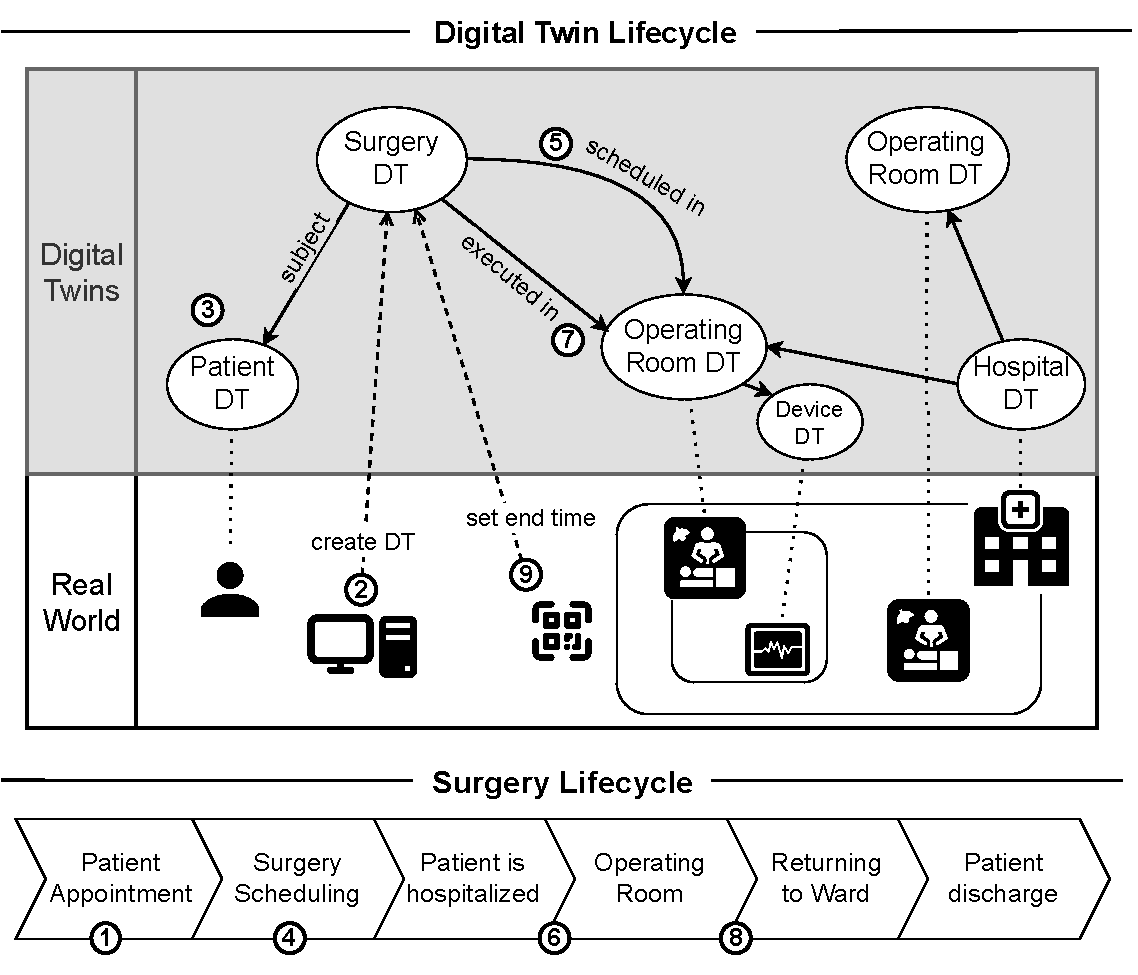
\includegraphics[width=\columnwidth]{figures/orm/DTORM.pdf}
    \caption{An example of how a DT ecosystem could support the management of ORs as well as the real-time tracking of elective surgery processes.}
    \label{fig:dt ecosystem}
\end{figure}

%When the process related to surgery starts, \emph{i.e.}, when the patient exits from the hospital ward, a dedicated DT is created to track and monitor the patient within the whole surgery process, collecting operations' periods and exposing information useful for the ORM tasks.
%
%In this perspective, the whole activities occurring within a surgery block -- not only limited to surgeries -- can be tracked and used to improve the ORM process.

%DTs can retrieve data about surgery rooms from the healthcare organisation's software systems. Moreover, the same software systems can provide information about the ongoing state of the surgeries.

The case study proposed in the next section describes a real-world architecture of a DT ecosystem for ORM implementing this overall picture.



%=======================================================
\section{Implemented Solution}
%=======================================================